\section{Introduction}

An engineer designing an inspection policy may need to specify how much testing the system should perform before deciding whether to repair or release an item. A standard partially observable Markov decision process (POMDP) values a test through its effect on expected task reward. A $\rho$-POMDP additionally rewards properties of the agent's belief, allowing information gain to have explicit value \citep{araya2010}. This introduces a practical choice: how much weight should information gain receive relative to reward?

We study a different design input, an expected sensing-usage target $B$. Such a target is useful when sensing is itself a deliverable, as in a coverage, monitoring, or verification requirement. It specifies the average number of tests or their expected cumulative cost. It is neither a hard limit on each episode nor an instruction to maximize reward subject to spending at most $B$. Those alternatives define different design problems, and our experiments measure the reward cost of meeting a target when reward alone would justify less sensing.

For a family of policies indexed by information weight $w$, let $U(w)$ be the expected sensing usage. We call the weight at which this curve crosses $B$ its \emph{operational shadow price}, $w^*(B)$. The adjective operational matters: this price is read from a usage curve, rather than obtained as the Lagrange multiplier of a usage-cap constraint. The curve can have plateaus, jumps, and non-monotone portions. A finite grid therefore estimates a crossing by a bracket. When the selected endpoint policies straddle a usage gap, a per-episode mixture can attain the target in expectation under the conditions of Definition~\ref{def:pi3}. The crossing threshold, its grid bracket, and this randomized policy are distinct objects.

Figures~\ref{fig:hero} and~\ref{fig:engineering_workflow} connect this construction to the engineer's workflow. The engineer supplies a model, states an expected-usage requirement, estimates the usage curve offline, and checks usage and reward on held-out episodes. During deployment the agent chooses each test or terminal decision from its current belief. It does not perform a prescribed number of tests on every item.

\begin{figure}[!t]
\centering
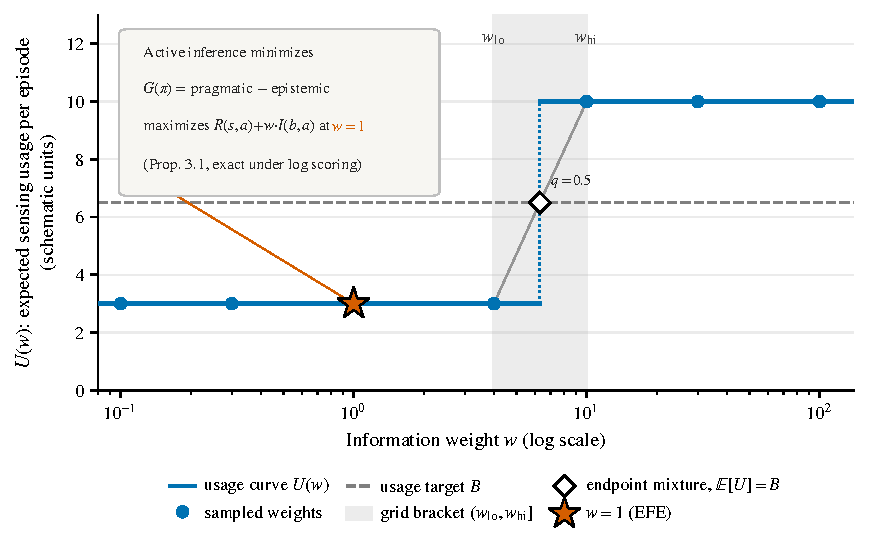
\includegraphics[width=\linewidth]{figures/fig_hero_price_curve_jair.pdf}
\caption{An expected-usage target selects a crossing of the usage curve (schematic). Sampled grid weights bracket a jump over $B$. The shaded band estimates the crossing threshold, while the diamond represents a mixture of the two endpoint policies that attains $B$ in expectation under Definition~\ref{def:pi3}. Its horizontal position is schematic, not a third deterministic weight. The information-unit default $w=1$ is one point on the curve and belongs to the level set of its own implicit budget. The equivalence shown in the inset uses the stated reward-based EFE objective, with exact reward identification under log scoring.}
\label{fig:hero}
\Description{A single line chart on a light background, with no photographic content. The horizontal axis is labeled information weight w and uses a log scale running from about 0.1 to 100. The vertical axis is labeled U of w, the expected sensing usage per episode in schematic units, running from 0 to about 13. A blue line stays flat at a low value of 3 from the left edge to a weight of about 6, jumps vertically there along a thin dotted blue riser to a high value of 10, and stays flat at 10 to the right edge. Seven blue dots mark the sampled grid weights at 0.1, 0.3, 1, 4, 10, 30, and 100, the first four on the low plateau and the last three on the high plateau. This single jump is drawn as a clean illustrative simplification, not as measured data, and usage curves reported elsewhere in this paper can include additional plateaus, jumps, or small non-monotone dips. A horizontal gray dashed line crosses the full width of the plot at a height of 6.5, between the two plateaus, representing a stated expected sensing budget B that no single sampled weight attains. A light gray vertical shaded band spans from the grid weight 4 up to and including the grid weight 10, labeled w-low and w-high near its top left and top right corners, marking the crossing bracket, the grid's estimate of where the curve crosses the budget. Where the dashed budget line meets the dotted riser, an open white diamond with a black outline marks the endpoint mixture, the randomized policy that plays w-high with probability q and w-low otherwise, and a small label beside it reads q equals 0.5. Two thin gray leader lines connect the diamond to the grid point at weight 4 on the low plateau and the grid point at weight 10 on the high plateau, the two endpoints it mixes. A black-outlined vermillion five-pointed star sits on the curve's low plateau at w equals 1, positioned clearly to the left of and outside the shaded band. A thin vermillion line connects the star to a small rounded text box in the upper left of the plot, an area with no curve or other data in it. The text box's right edge stops with a clear gap of open space before the shaded band's left edge. The text box states, on four lines, that minimizing Expected Free Energy, written as G of pi equals a pragmatic term minus an epistemic term, is exactly equivalent to maximizing a rho-POMDP objective, reward of s and a plus w times information gain of b and a, at w equals 1, and that this identity is exact under log scoring rules, citing the equivalence proposition by number. Within that box, only the text w equals 1 is printed in the same vermillion color as the star, and every other word in the box is plain dark text. A frameless legend in three columns below the plot lists six items, the blue curve, the sampled grid weights, the dashed budget line labeled as a target, the shaded crossing bracket labeled as a grid estimate, the endpoint mixture diamond with its expected usage equal to B, and the star. Read together, the figure shows expected sensing usage jumping with an information-gain weight, a stated budget falling in the gap so that the sampled grid can only bracket the crossing, a separate randomized mixture of the two bracket endpoints attaining the budget in expectation, and a single labeled point on the same curve, the weight that active inference derives on its own, shown as forced by a theorem rather than chosen by hand, and shown sitting outside the particular bracket drawn here rather than coinciding with it.}
\end{figure}

\begin{figure}[!t]
\centering
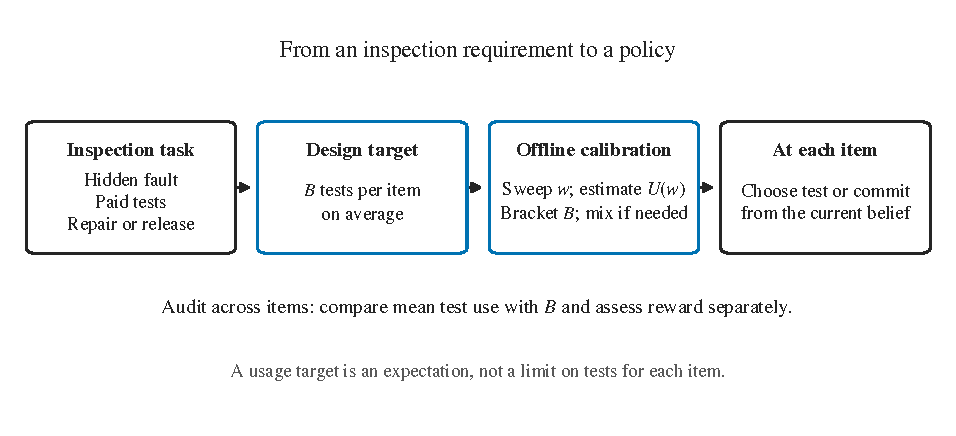
\includegraphics[width=\linewidth]{figures/fig_engineering_workflow.pdf}
\caption{From an inspection requirement to a running policy (schematic, not experimental data). For a state-preserving task with a hidden fault and paid tests, the engineer states a target $B$ in expected tests per item. An offline sweep estimates usage $U(w)$ and brackets $B$. When a usage gap lies between the selected endpoint policies, mixing them across items can meet the target under Definition~\ref{def:pi3}'s conditions. The deployed agent chooses tests and terminal actions from its current belief. Usage and reward are assessed separately: meeting $B$ does not establish reward optimality under a sensing cap.}
\label{fig:engineering_workflow}
\Description{A four-stage horizontal flow chart headed From an inspection requirement to a policy. The boxes read: Inspection task, hidden fault, paid tests, repair or release. Design target, B tests per item on average. Offline calibration, sweep information weight w, estimate usage U of w, bracket B and mix if needed. At each item, choose test or commit from the current belief. Arrows connect the boxes left to right. Below them a line says to audit mean test use against B and assess reward separately. A final line says the usage target is an expectation rather than a limit on tests for each item.}
\end{figure}

The price has a useful response to a change of reward units. Multiplying all rewards and costs by $\alpha>0$ and the information weight by the same factor preserves the receding-horizon planner's decisions under the assumptions of Proposition~\ref{prop:pi1}. Observation counts are unchanged and cumulative sensing costs rescale by $\alpha$. An online feedback rule can also adjust the weight when observed usage differs from the target. We prove stationary convergence for its projected, decaying-step form under explicit conditions and separately evaluate re-adaptation after a reward-scale shift.

Active inference identifies a particular point in this policy family. Its Expected Free Energy (EFE) objective combines pragmatic value with expected information gain \citep{friston2010,parr2019}. For the recursive, reward-based objective specified here, minimizing EFE is equivalent to maximizing reward plus information gain at $w=1$. The reward--information identification is exact under log scoring \citep{bernardo1979}. For ordinary task rewards it depends on the declared reward convention and the treatment of the preference normalizer. The coefficient is therefore an untuned default under shared units, not a scale-invariant calibration. In particular, $w=1$ belongs to the level set of its implicit budget $U(1)$, but need not equal that budget's crossing threshold.

The paper makes three contributions. First, it formulates expected-usage calibration within a $\rho$-POMDP policy family, distinguishing the level set, crossing threshold, grid estimate, and endpoint mixture. It establishes scale equivariance and a conditional stationary-convergence result for online control. Second, it proves the EFE equivalence for observe-then-commit problems and extends it to the hidden-state-preserving actions of factored observation POMDPs. A two-state analysis characterizes sensing onset and an interval of weights that avoids an unnecessary second observation. Third, it evaluates the calibration procedure and the information-unit default against reward-only planning, tuned information gain, POMCP, and near-optimal offline references. Code and experiment data are available at \url{https://github.com/PatrickAllenCooper/rho_aif}.

The evidence also sets limits on these contributions. Targets selected by a predeclared rule from calibration curves are met on held-out seeds to within $0.13$ observations, but the selected mixtures can sacrifice reward relative to a constrained reference and need not be the best mixtures in the weight family. The untuned $w=1$ lies in the reward-maximizing bracket on three of five swept environments and is beaten on the other two. Its advantage over reward-only planning depends on the observation structure and available planning depth, rather than on state-space size alone. Ordinary information gain can spend the budget on uncertainty unrelated to reward, and the stated equivalence does not cover observation actions that change the hidden state. These limitations remain part of the main argument, with full controls and counterexamples in the appendices.

An abridged version was accepted at IWAI 2026 \citep{cooper2026iwai}. It contains the EFE equivalence results and their benchmark evaluation. The budgeted formulation, scale-equivariance and controller results, budget experiments, and distractor and destructive-sensing analyses are extensions. We also revise the workshop version's claim that the advantage grows with state-space size and observation-action count, which RockSample[11,11] does not support.

Section~\ref{sec:methodology} defines the model and EFE objective. Section~\ref{sec:budget} develops usage calibration, and Section~\ref{sec:experiments} specifies the evaluation protocol. Sections~\ref{sec:budget_experiments} and~\ref{sec:results} report the budget and EFE results. Section~\ref{sec:discussion} explains their practical scope. Appendices retain proofs, complete tables, robustness studies, and implementation details.
